\chapter{Theoretical Foundations\label{cha:chapter3}}

This chapter describes the implementation of component X.

\section{Convolutional Neural Networks}

\section{Transformer Models}

\section{Arithmetic Coding}
Arithmetic coding is an algorithm used for entropy coding, that is a technique for encoding and decoding a sequence of symbols in an efficient way \citep{witten_arithmetic_1987}. As an example, a string of characters can be considered. A standard non-optimized way of storing a string is by using the \ac{ascii} encoding which used a fixed seven bytes per character of the string. Entropy coding algorithms improve on this by allocating fewer bits to more common characters and therefore more bits to less common characters \citep{witten_arithmetic_1987}. In total, this leads to a lower number of required bits for the total message, given an accurate probability model for the frequencies of the characters. In fact, if the provided probability model is perfectly accurate, arithmetic coding yields an encoding close to an optimal encoding, that is an encoding that uses a number of bits equal to the entropy of the encoded input \citep{witten_arithmetic_1987}. This is the fewest number of bits possible for a lossless encoding of an arbitrary message, which was proven with Shannon's source coding theorem \citep{shannon_mathematical_1948,mackay_information_2003}.

\begin{figure}
\centering
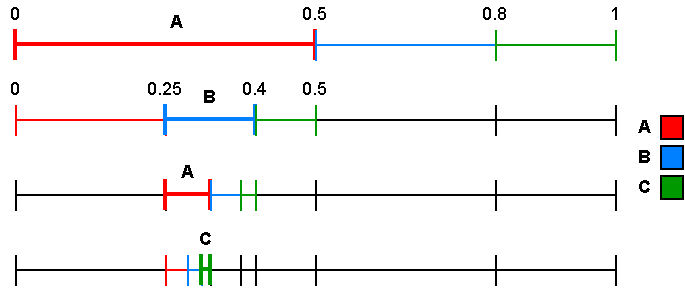
\includegraphics[scale=1]{ArithmeticCoding.pdf}
\caption{Arithmetic coding process of "ABAC".}
\label{fig:arithmetic}
\end{figure}

Arithmetic coding, using the theoretical version of the algorithm, works by encoding the entire input message into one arbitrary-precision rational number $q$ with $0 \leq q < 1$ \citep{said_introduction_2023}. In practice the algorithm is slightly modified to account for the lack of infinite precision in computers, as will be detailed later in this section. The encoding is performed using an iterative process. In order to understand this process, consider for an example an alphabet consisting of three symbols, 'A', 'B' and 'C' with 'A' having the probability $0.5$, 'B' having the probability $0.3$ and therefore 'C' having the probability $0.2$. Encoding an message is performed symbol by symbol. To encode the first symbol, the interval $[0,1)$ (meaning numbers $a$ with $0 \leq a < 1$) is split into three parts according to these probabilities. If the first symbol is 'A', the final encoding number $q$ will be in the interval $[0,0.5)$. Likewise, if the first symbol is 'B' or 'C', $q$ will be in the intervals $[0.5,0.8)$ or $[0.8,1)$ respectively. The second symbol is then encoded by splitting the interval determined from the first symbol again, using the same probabilities. A sequence of two 'A' symbols would therefore result in $q$ being in the interval $[0,0.25)$. This procedure is iterated until each symbol of the input message is encoded, resulting in a single number $q$ representing the entire input. This process can be seen in \autoref{fig:arithmetic} using the aforementioned probabilities for the word "ABAC". This number encodes the original message nearly optimally given a perfect probability distribution, with a difference of less than a bit to the entropy of the message. The reason for this discrepance is that $q$ is always represented using an integer amount of bits. If the input image has a non-integer entropy, the required amount of bits to store $q$ is the entropy rounded up to the nearest integer. However, the complete algorithm of arithmetic encoding requires an additional source of information that needs to be transmitted to the decoder. In order to decode the message, the decoder needs to know the probability model as well as a way to distinguish when the message ends. The first is constant with respect to message length. The second can be transferred using only logarithmic overhead with respect to message length. This is often done by adding an additional token that signifies the end of the message \citep{said_introduction_2023}.
As mentioned before, the algorithm is adapted slightly in practice in order to use fixed precision numbers instead of arbitrary precision numbers. Rounding operations as a result of using fixed point numbers are the same for encoder and decoder and therefore do not inhibit the algorithm in principle. However, as a result of rounding, intervals can become small enough that they are not representable with fixed point numbers of the used precision. In this case, the intervals are changed in a determinable way so that they are again representable. This process is called renormalization and multiple algorithms to perform this procedure exist.
Arithmetic coding also allows for the possibility of changing the probability distribution during the encoding process based on previously encoded symbols. This is possible because the decoder decodes the symbols in the same order as the encoder encodes them and can therefore perform the same change to the probability distribution as the encoder, as long as the method for changing the probability model was decided beforehand \citep{said_introduction_2023}.

In learning-based lossy image compression, arithmetic coding is used as part of the Hyperprior architecture order to encode the latent representation of an input image \citep{balle_end--end_2017,minnen_joint_2018,balle_variational_2018}. The latent representation of the input image and the probability distribution used for the arithmetic coder can be learned using \acp{ann}.

\section{Hyperprior Architecture}